\section{Analysis and Design} \label{sec:Design}

Seeing that this is a system dealing with finance, it would make sense to treat
the categories as if they were accounts. And, in order to make sure to imbue
this system with knowledge acquired by more experienced programmers, it makes
sense to make use of analysis and design patterns.

%TODO: maybe move to appendix
It is also useful at this point to make a distinction between the types of
classes used to model the domain between three possible kinds: the first are
the classes which model the interaction between the system and its actors --
these are called \emph{boundary classes}; the second kind are those classes
which model information and/or behaviour or some concept or phenomenon -- these
will be called \emph{entity classes}; and lastly, there are those classes which
model transactions, coordination, control and sequencing of other objects --
which are known as \emph{control classes} (Jacobson et al., 1999,
\cite[cited][pp.~198-201]{bennett2010object}).

The first analysis patterns which seem appropriate are a modified version of
the \emph{Account} pattern, used to create the \texttt{Category} entity class,
and the \emph{Quantity} pattern for the \texttt{Amount} entity class
(\cite[][Sections~6.1~\&~3.1]{fowler1997analysis}):
\begin{figure}[ht!]
  \begin{center}
    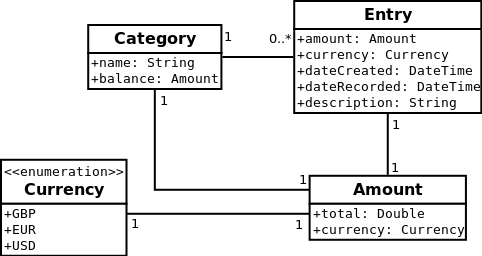
\includegraphics[width=9cm]{./contents/img/Class_Diagram_-_Categories_and_Amount.png}
  \end{center}
  \caption{}
  \label{fig:ClassDiagram.CategoriesAndAmount}
\end{figure}
\FloatBarrier

As implied by the diagram above, the \texttt{Category} class will be associated
with instances of the \texttt{Entry} class. This is done so that the only way to
change the total of a category is by adding positive or negative entries to it
-- for example, to indicate a credit to a category, a negative entry can be
added to it. The modification to the original Account pattern consists of the
fact that, whereas in the original pattern an instance of \texttt{Account}
would keep track of the balance, there is no need to keep track of the current
balance in each \texttt{Category} -- the purpose of the system is to allow the
user to view a summary of income/expenditure by period, so this will have to be
calculated each time.

Another design choice which can be observed in Figure
\ref{fig:ClassDiagram.CategoriesAndAmount} is that the \texttt{Amount} class
also possesses an attribute for currency. This has been designed so as to allow
for the possibility of extending the system to keep track of transactions in
multiple currencies, although this was not a specific requirements. Initially,
there will only be a single default currency which shall be set at runtime.

The next step is to provide a way for these entries to be added to categories.
For this to happen, there needs to be a constraint to ensure that double entry
happens every time a change needs to be made to a category. One of the ways to
achieve this is to apply the \emph{Transaction} pattern
(\cite[][Section~6.2]{fowler1997analysis}):
\begin{figure}[ht!]
  \begin{center}
    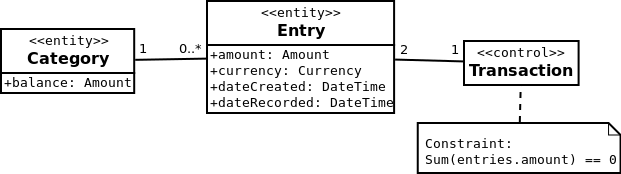
\includegraphics[width=9cm]{./contents/img/Class_Diagram_-_Transaction.png}
  \end{center}
  \caption{}
  \label{fig:ClassDiagram.Transaction}
\end{figure}
\FloatBarrier


Furthermore, especially due to the requirements for tax estimates, the
\emph{Summary Accounts} pattern (\cite[][Section~6.3]{fowler1997analysis}) will
be adapted to help classify categories between income and expenditure. A
\texttt{SummaryCategory} implements the \texttt{Category} interface, and would
implement its \texttt{getEntries} method so that its entries are those of its
components. It's components are other instances of \texttt{Category}, so they
can be both both \texttt{DetailCategory} and its own type -- the implementation
will have to take this into account somehow, such as by using recursion. The
class diagram below (Figure \ref{fig:ClassDiagram.SummaryCategory}) can
illustrate it better:

\textbf{TODO}

\begin{figure}[ht!]
  \begin{center}
    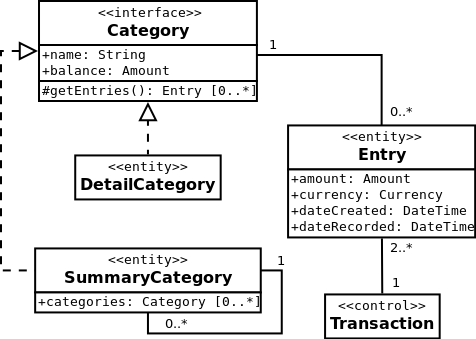
\includegraphics[width=11cm]{./contents/img/Class_Diagram_-_Summary_Category.png}
  \end{center}
  \caption{}
  \label{fig:ClassDiagram.SummaryCategory}
\end{figure}
\FloatBarrier


Lastly, also as a preparation for the estimate tax functionality, it would be
useful to design them based on the \emph{Memo Account} and \emph{Posting Rules}
patterns (\cite[][Section~6.4~\&~6.5]{fowler1997analysis}).

\textbf{TODO: implement the Memo Account and Posting Rules, and employ textual descriptions}


After having determined the analysis patterns which shall be employed, it makes
sense to dive into a deeper analysis of the use cases described in Chapter
\ref{sec:Requirements}. At this point the objective will be to start modelling
classes based on concepts or things found in the problem domain. This will be
done in the following subsections.

\subsection{Create Manual Entry} \label{sec:AnalysisAndDesign.ManualEntry}

%TODO: check if this diagram still makes sense after implementation
The \emph{Create Manual Entry} use case, which allows a
user to input financial transactions individually using a specific interface,
can be modelled as follows (Figure \ref{fig:CommDiagram.CreateManualEntry}):
\begin{figure}[ht!]
  \begin{center}
    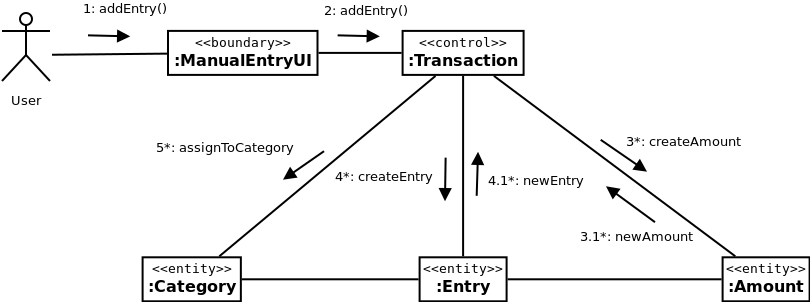
\includegraphics[width=12cm]{./contents/img/Comm_Diagram_-_Manual_Entry.png}
  \end{center}
  \caption{Communication Diagram for the \emph{Create Manual Entry} use case}
  \label{fig:CommDiagram.CreateManualEntry}
\end{figure}
\FloatBarrier

As the diagram above indicates, the \texttt{Transaction} class is responsible for
the creation of new instances of \texttt{Entry} and \texttt{Amount}, which then get
assigned to the \texttt{Category} instances chosen, or created, by the user.
Once the user starts typing, the \texttt{CategorySuggester} is triggered to
suggest categories. The actual implementation of how this suggestions happen
may vary, but initially it should at least be based on what the user types in
the search box. If the user chooses to create a new category instead, then they
will be taken to the appropriate interface to allow them to do so. Once the
user is satisfied and chooses to submit, the system will start to input the
transactions in the appropriate category or categories.

Although \texttt{Transaction} was originally thought of as a \emph{control
class}, it was later decided that it would be beneficial to save the
transaction information, so it was made into an \emph{entity class} instead.
It is also worth noting that, although implicit in the diagram and the
wireframe on Figure \ref{fig:Wireframe.CreateManualEntry}, it is estimated that
the user will start the interface, enter the transaction's details, and then
start the process to find a category. Seeing that there will be a search
suggestion at this point, it felt it was appropriate to have the diagram on
Figure \ref{fig:CommDiagram.CreateManualEntry} have its first message sent at
this stage.

It is also important to emphasise the fact that \texttt{CategorySuggester} is
only an interface at this point, and that the suggester in the diagram will be
any object which implements this interface. This is to allow more flexibility
in the implementation of the classes responsible for suggesting categories to
the user.

\subsection{Upload Statement} \label{sec:AnalysisAndDesign.UploadStatement}

The user should be able to upload their bank statements, provided that they are
in a suitable format. The specifics of the format will be described in the
implementation phase, together with more information on how to encapsulate as
much as possible the complexities related to the formatting of this
information.  For the analysis and design phases, the emphasis will be on
modelling the objects and their interactions. The diagram (Figure
\ref{fig:CommDiagram.CreateManualEntry}) below illustrates this process:
\begin{figure}[ht!]
  \begin{center}
    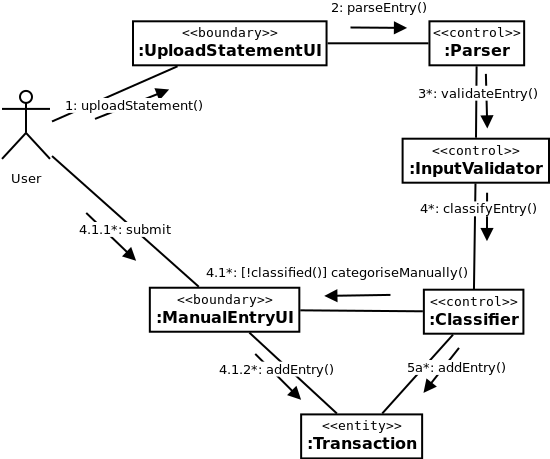
\includegraphics[width=14cm]{./contents/img/Comm_Diagram_-_Upload_Statement.png}
  \end{center}
  \caption{Communication Diagram for the \emph{Upload Statement} use case}
  \label{fig:CommDiagram.CreateManualEntry}
\end{figure}
\FloatBarrier

As can be seen in the diagram above, the process is spread among many classes.
After the user uploads the statement, the loaded raw input will be sent to a
\texttt{Parser} which will separate it according to the columns into the
appropriate fields and line items. Then, what is now a collection of statement
line items will be passed on to an \texttt{InputValidator} to make sure the user
input is valid. Lastly, the resulting validated entries will be sent down to a
\texttt{Classifier}, which will signal the relevant \texttt{Transaction}
instance(s) to add the entries to their relevant \texttt{Category} instances --
this last part has already been illustrated in Figure
\ref{fig:CommDiagram.CreateManualEntry}. 

When the \texttt{Classifier} cannot match a line item against any of the existing
categories, it will pass the line in question to the \texttt{ManualEntryUI},
which, apart from having all transaction details already populated, will rely
on the process described at subsection \ref{sec:AnalysisAndDesign.ManualEntry}
to properly categorise the item and then forward it to \texttt{Transaction} to
create the categories.

\subsection{Visualise Categorised Summary} \label{sec:AnalysisAndDesign.ViewSummary}
As mentioned before, this feature will allow the user to view a summary of
their income and expenditure by category.  The user will enter the period which
they want to examine, and the system will retrieve the categories which have
entries with those dates.  The system should then sort the categories by income
or expenditure and by total, and then display it to the user. Optionally, the
user can filter the output further by choosing a single category.

Below (Figure \ref{fig:CommDiagram.VisualiseCategorisedSummary}) is a
communication diagram to illustrate this interaction: 
\begin{figure}[ht!]
  \begin{center}
    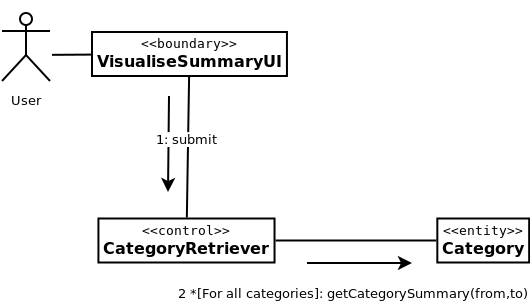
\includegraphics[width=12cm]{./contents/img/Comm_Diagram_-_Visualise_Categorised_Summary.png}
  \end{center}
  \caption{communication diagram for \emph{Visualise Categorised Summary} use case}
  \label{fig:CommDiagram.VisualiseCategorisedSummary}
\end{figure}
\FloatBarrier



\subsection{Calculate Budget} \label{sec:AnalysisAndDesign.CalculateBudget}
This feature will allow the user to request the system to calculate a budget
for them over a period of time. What the system will do then is retrieve all
categories over the last 12 months, then calculate their means and take them as
ratio of the income over the same last period. Then, it will take the first few
which make up more than 80\% of the total, and add all the others which make up
the remainder and add them up as `other' or something similar. It will then
show these totals to the user, in a similar way as it shows the categorised
summary. The communication diagram below (Figure
\ref{fig:CommDiagram.CalculateBudget}) illustrates the steps taken by the
application layer.
\begin{figure}[ht!]
  \begin{center}
    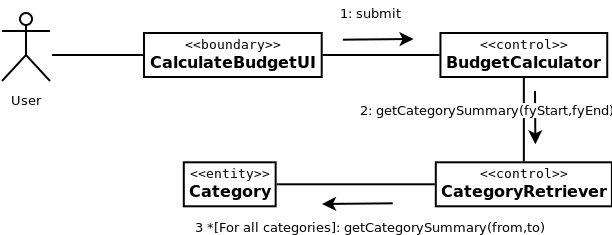
\includegraphics[width=14cm]{./contents/img/Comm_Diagram_-_Calculate_Budget.png}
  \end{center}
  \caption{communication diagram for \emph{Calculate Budget}}
  \label{fig:CommDiagram.CalculateBudget}
\end{figure}
\FloatBarrier



\subsection{Estimate Tax} \label{sec:AnalysisAndDesign.EstimateTax}

%TODO: refer to
%\cite[][location~2071-rest~of~chapter~6~and~maybe~chapter~7]{fowler1997analysis}
%as these patterns seem like they would be useful here.
This feature will allow the user to calculate an estimate of the amount of tax
due for a financial year, based on their income and expenditure. For this to
happen, the user will have to provide the date when the financial year begins,
and the tax tiers in their country. This is loosely based on UK Generally
Accepted Accounting Practices (UK GAAP), where taxation is centralised and
happens in tiers. The communication diagram of figure
\ref{fig:CommDiagram.EstimateTax} exemplifies the application module which will
model this functionality:

\textbf{TODO}

\begin{figure}[ht!]
  \begin{center}
    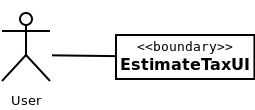
\includegraphics[width=5cm]{./contents/img/Comm_Diagram_-_Estimate_Tax.png}
  \end{center}
  \caption{}
  \label{fig:CommDiagram.EstimateTax}
\end{figure}
\FloatBarrier
